\documentclass[bachelor, och, labwork]{shiza}
% параметр - тип обучения - одно из значений:
%    spec     - специальность
%    bachelor - бакалавриат (по умолчанию)
%    master   - магистратура
% параметр - форма обучения - одно из значений:
%    och   - очное (по умолчанию)
%    zaoch - заочное
% параметр - тип работы - одно из значений:
%    referat    - реферат
%    coursework - курсовая работа (по умолчанию)
%    diploma    - дипломная работа
%    pract      - отчет по практике
% параметр - включение шрифта
%    times    - включение шрифта Times New Roman (если установлен)
%               по умолчанию выключен
\usepackage{subfigure}
\usepackage{tikz,pgfplots}
\pgfplotsset{compat=1.5}
\usepackage{float}

%\usepackage{titlesec}
\setcounter{secnumdepth}{4}
%\titleformat{\paragraph}
%{\normalfont\normalsize}{\theparagraph}{1em}{}
%\titlespacing*{\paragraph}
%{35.5pt}{3.25ex plus 1ex minus .2ex}{1.5ex plus .2ex}

\titleformat{\paragraph}[block]
{\hspace{1.25cm}\normalfont}
{\theparagraph}{1ex}{}
\titlespacing{\paragraph}
{0cm}{2ex plus 1ex minus .2ex}{.4ex plus.2ex}

% --------------------------------------------------------------------------%


\usepackage[T2A]{fontenc}
\usepackage[utf8]{inputenc}
\usepackage{graphicx}
\graphicspath{ {./images/} }
\usepackage{tempora}

\usepackage[sort,compress]{cite}
\usepackage{amsmath}
\usepackage{amssymb}
\usepackage{amsthm}
\usepackage{fancyvrb}
\usepackage{listings}
\usepackage{listingsutf8}
\usepackage{longtable}
\usepackage{array}
\usepackage[english,russian]{babel}

\usepackage[colorlinks=false]{hyperref}
\usepackage{url}

\usepackage{underscore}
\usepackage{setspace}
\usepackage{indentfirst} 
\usepackage{mathtools}
\usepackage{amsfonts}
\usepackage{enumitem}
\usepackage{tikz}
\usepackage{verbatim}
\usepackage{minted}

\newcommand{\eqdef}{\stackrel {\rm def}{=}}
\newcommand{\specialcell}[2][c]{%
\begin{tabular}[#1]{@{}c@{}}#2\end{tabular}}

\renewcommand\theFancyVerbLine{\small\arabic{FancyVerbLine}}

\newtheorem{lem}{Лемма}

\begin{document}

% Кафедра (в родительном падеже)
\chair{теоретических основ компьютерной безопасности и криптографии}

% Тема работы
\title{Алгоритм Флойда-Уоршелла}

% Курс
\course{3}

% Группа
\group{331}

% Факультет (в родительном падеже) (по умолчанию "факультета КНиИТ")
\department{факультета КНиИТ}

% Специальность/направление код - наименование
%\napravlenie{09.03.04 "--- Программная инженерия}
%\napravlenie{010500 "--- Математическое обеспечение и администрирование информационных систем}
%\napravlenie{230100 "--- Информатика и вычислительная техника}
%\napravlenie{231000 "--- Программная инженерия}
\napravlenie{100501 "--- Компьютерная безопасность}

% Для студентки. Для работы студента следующая команда не нужна.
% \studenttitle{Студентки}

% Фамилия, имя, отчество в родительном падеже
\author{Токарева Никиты Сергеевича}

% Заведующий кафедрой
% \chtitle{} % степень, звание
% \chname{}

%Научный руководитель (для реферата преподаватель проверяющий работу)
\satitle{доцент} %должность, степень, звание
\saname{А. Н. Гамова}

% Руководитель практики от организации (только для практики,
% для остальных типов работ не используется)
% \patitle{к.ф.-м.н.}
% \paname{С.~В.~Миронов}

% Семестр (только для практики, для остальных
% типов работ не используется)
%\term{8}

% Наименование практики (только для практики, для остальных
% типов работ не используется)
%\practtype{преддипломная}

% Продолжительность практики (количество недель) (только для практики,
% для остальных типов работ не используется)
%\duration{4}

% Даты начала и окончания практики (только для практики, для остальных
% типов работ не используется)
%\practStart{30.04.2019}
%\practFinish{27.05.2019}

% Год выполнения отчета
\date{2022}

\maketitle

% Включение нумерации рисунков, формул и таблиц по разделам
% (по умолчанию - нумерация сквозная)
% (допускается оба вида нумерации)
% \secNumbering

%-------------------------------------------------------------------------------------------

\tableofcontents


\section{Описание алгоритма}

  Этот алгоритм был одновременно опубликован в статьях Роберта Флойда (Robert Floyd) и Стивена Уоршелла (Варшалла) (Stephen Warshall) в 1962 г., по имени которых этот алгоритм
  и называется в настоящее время. Впрочем, в 1959 г. Бернард Рой (Bernard Roy) опубликовал практически такой же алгоритм, но его публикация осталась незамеченной.
  Алгоритм Флойда (или Флойда-Уоршелла, Floyd–Warshall) позволяет найти кратчайшее расстояние между любыми двумя вершинами в графе, при этом веса ребер 
  могут быть как положительными, так и отрицательными. Данный алгоритм также использует идею динамического программирования.
  
  Будем считать, что в графе $n$ вершин, пронумерованных числами от $0$ до $n-1$. Задана матрица $D$
  весов ребер графа. Если в матрице в $i$-й строке в $j$-м столбце стоит 0, то это означает, что
  дуги из вершины $i$ в вершину $j$ нет. Однако при вводе данной матрицы $D$ все нулевые значения
  значения будут равны бесконечности $\infty$. Также будем считать, что $d_{ii} = 0$.

  Ключевая идея алгоритма -- разбиение процесса поиска кратчайших путей на 
 
  Перед $k$-ой ($0 \leq k \leq n-1$) фазой величина $d_{ij}$ равна длине кратчайшего пути из вершины $i$ в вершину $j$, если этому пути разрешается заходить только в вершины с номерами, меньшими $k$ (начало и конец пути не считаются).
  
  Пусть теперь мы находимся на $k$-й фазе, и хотим пересчитать матрицу $D$ таким образом, чтобы она соответствовала требованиям уже для $k+1$-ой фазы. Зафиксируем какие-то вершины $i$ и $j$. У нас возникает два принципиально разных случая:
  
  \begin{itemize}
    \item Кратчайший путь из вершины $i$ в вершину $j$, которому разрешено дополнительно проходить через вершины $\{ 0, 1, \ldots, k \}$, совпадает с кратчайшим путём, которому разрешено проходить через вершины множества $\{ 0, 1, \ldots, k-1 \}$.
    
    В этом случае величина $d_{ij}$ не изменится при переходе с $k$-й на $k+1$-ю фазу.
    \item "Новый" кратчайший путь стал лучше "старого" пути.
    
    Это означает, что "новый" кратчайший путь проходит через вершину $k$. Сразу отметим, что мы не потеряем общности, рассматривая далее только простые пути (т.е. пути, не проходящие по какой-то вершине дважды).
  \end{itemize}
 
 Тогда заметим, что если мы разобьём этот "новый" путь вершиной $k$ на две половинки (одна идущая $i \Rightarrow k$, а другая -- $k \Rightarrow j$), то каждая из этих половинок уже не заходит в вершину $k$. Но тогда получается, что длина каждой из этих половинок была посчитана ещё на $k-1$-ой фазе или ещё раньше, и нам достаточно взять просто сумму $d_{ik} + d_{kj}$, она и даст длину "нового" кратчайшего пути.
 
 Таким образом, вся работа, которую требуется произвести на $k$-ой фазе — это перебрать все пары вершин и пересчитать длину кратчайшего пути между ними. В результате после выполнения $n$-ой фазы в матрице расстояний $d_{ij}$ будет записана длина кратчайшего пути между $i$ и $j$, либо $\infty$, если пути между этими вершинами не существует.


  \section{Код программы, реализующий алгоритм}

  Далее представлена реализация алгоритма Флойда, написанная на языке $C++$.

  
  \inputminted[fontsize=\small]{C++}{code/floyd.cpp}

  Далее приведем несколько примеров, подав некоторые случайные числа в качестве входных данных, чтобы проверить корректность, написанного
  кода.

  На рисунке 1 представлен неориентированный взвешенный граф из 6 вершин. Из рисунка 2 видно, что поиск кратчайших путей сработал корректно.

  \begin{figure}[H]
    \centering
    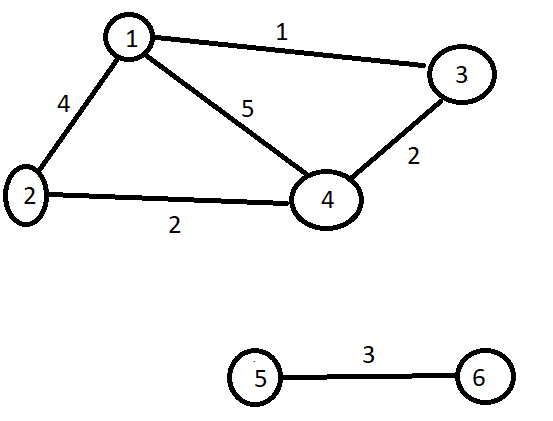
\includegraphics[width=0.8\textwidth]{img/2_1}
    \caption{Взвешенный неориентированный граф}
  \end{figure}

  \begin{figure}[H]
    \centering
    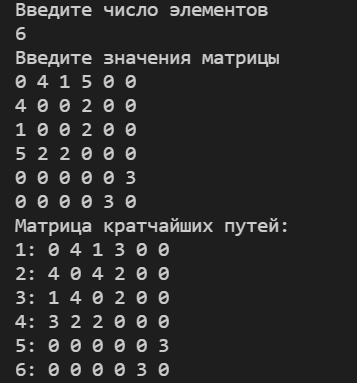
\includegraphics[width=0.8\textwidth]{img/2_2}
    \caption{Результат работы алгоритма}
  \end{figure}

  На рисунке 3 представлен ориентированный взвешенный граф из 6 вершин.


  \begin{figure}[H]
    \centering
    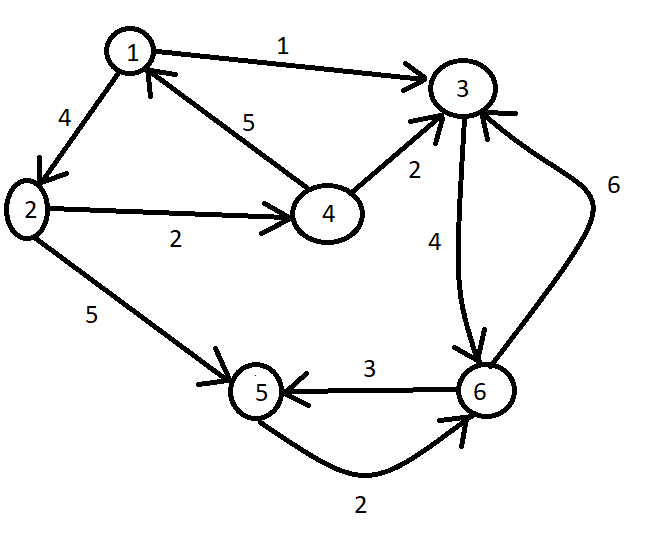
\includegraphics[width=0.8\textwidth]{img/2_3}
    \caption{Взвешенный ориентированный граф}
  \end{figure}
  
  А на рисунке 4 показан результат работы алгоритма Флойда.
  \begin{figure}[H]
    \centering
    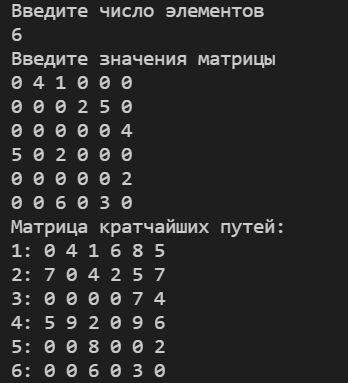
\includegraphics[width=0.8\textwidth]{img/2_4}
    \caption{Результат работы алгоритма}
  \end{figure}

  \section{Анализ алгоритма}

  Очевидно, что сложность данного алгоритма равна $O(n^3)$, так как здесь используется три вложенных друг в друга цикла,
  в которых реализуется пересчитывание кратчайших путей.

  Стоит отметить, что Алгоритм Флойда некорректно работает при наличии цикла отрицательного веса, но при этом если путь 
  от $i$ до $j$ не содержит цикла отрицательного веса, то вес этого пути будет найден алгоритмом правильно. Также при помощи
  данного алгоритма можно определить наличие цикла отрицательного веса: если $i$ вершина лежит на цикле отрицательного 
  веса, то значение $d_{ii}$ будет отрицательным после окончания алгоритма.

\conclusion

В данной лабораторной работе был рассмотрен алгоритм Флойда - Уоршелла и был проведен анализ оценки его сложности.
Это послужило созданием её программной реализации, написанной на языке $C++$. 

\begin{thebibliography}{3}
  \bibitem{1}
  Статья "Алгоритм Флойда-Уоршелла"  / [Электронный ресурс] URL: https://ru.wikipedia.org/wiki/Алгоритм_Флойда_—_Уоршелла (дата обращения 26.02.2022), Яз. рус
  \bibitem{2}
  Статья "Алгоритм Флойда-Уоршелла нахождения кратчайших путей между всеми парами вершин" / [Электронный ресурс] URL: https://e-maxx.ru/algo/floyd_warshall_algorithm (дата обращения 26.02.2022), Яз. рус.
  \bibitem{3}
  Стивен С. Скиен, "Алгоритмы. Руководство по разработке 2-е издание" / Санкт-Петербург: БХВ-Петербург, 2021 г., Яз. рус.   
\end{thebibliography}

\end{document}
